
La figure suivante présente les différents prototypes d'interface réalisés à la main. Pour valider les concepts et faire une première itération corrective suite aux remarques formulées lors de la présentation de nos interfaces. \\

\begin{figure}[H]
    \label{fig-mockup1}
    \noindent\makebox[\textwidth]{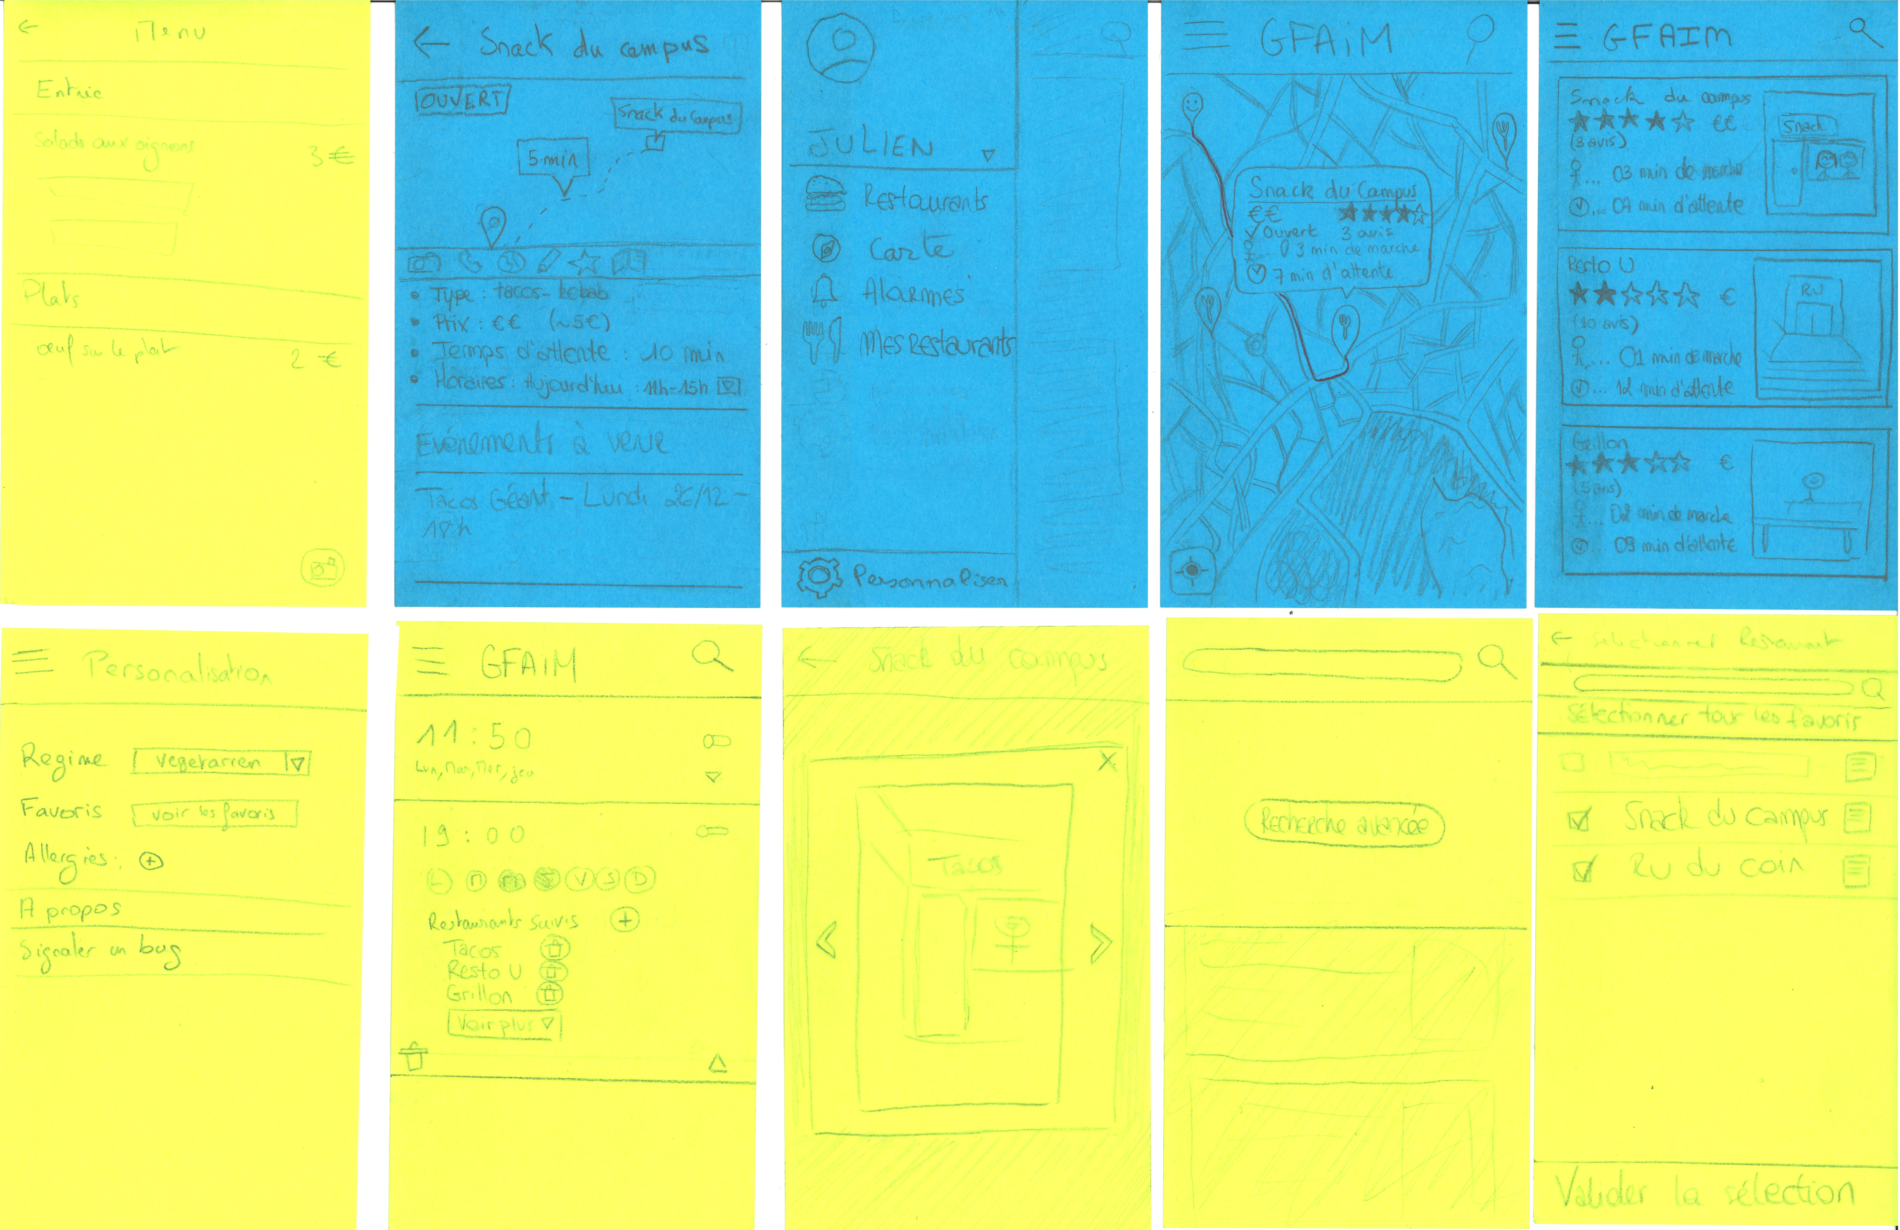
\includegraphics[width=15cm]{figures/mockups_1.png}}
    \noindent\makebox[\textwidth]{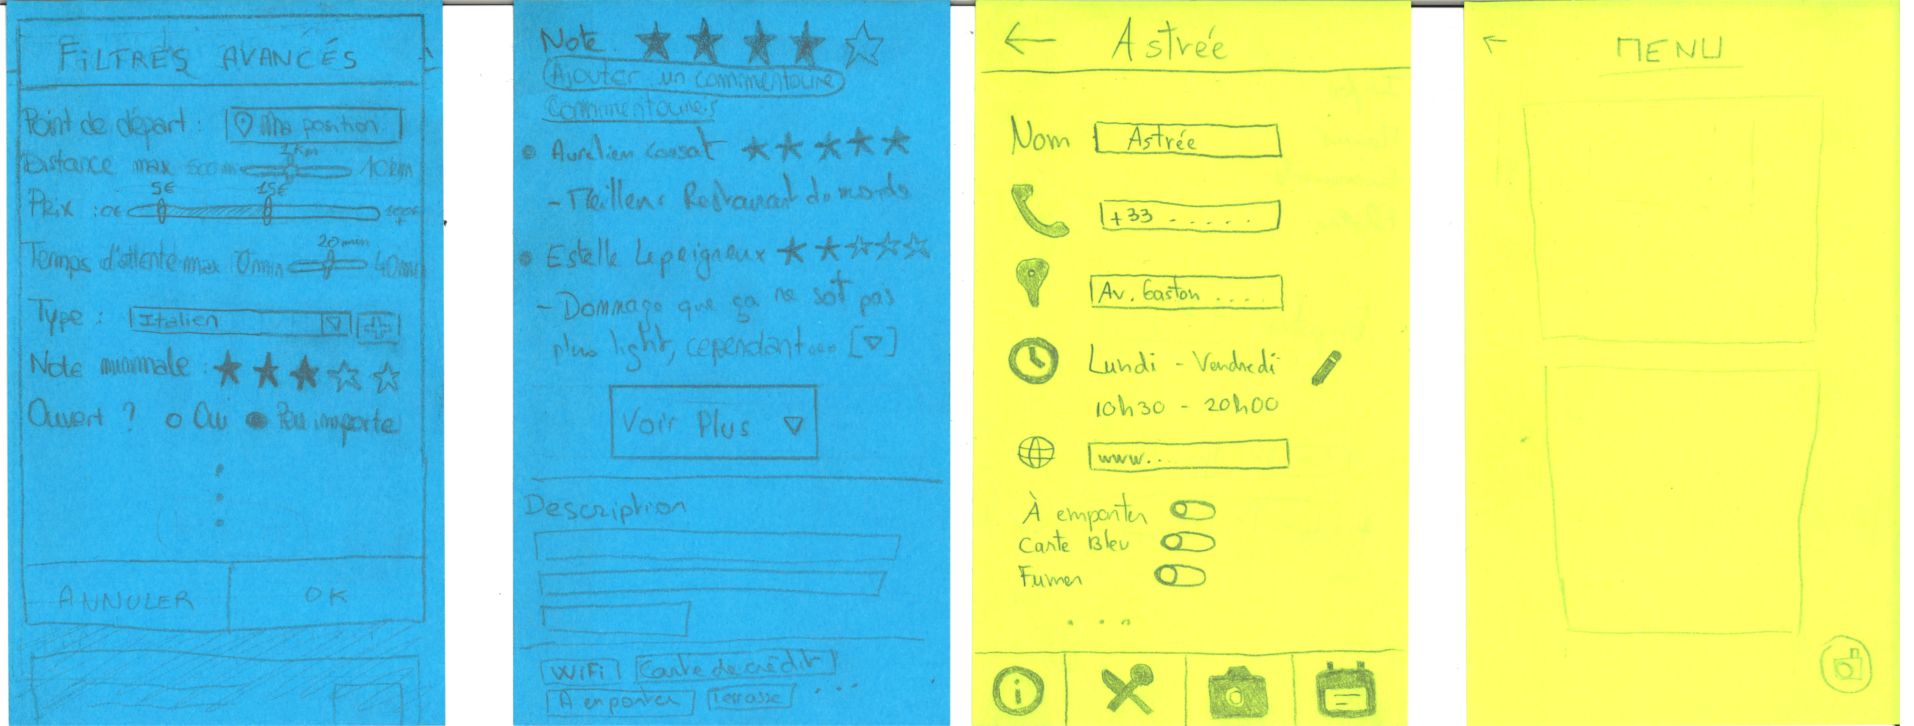
\includegraphics[width=15cm]{figures/mockups_2.png}}
    \caption{Mockups}
\end{figure}

Ces interfaces ont été réalisées sur des Post-It de la taille d'un écran de smartphone afin de nous placer dans les conditions réelles de taille et nous permettre de dimensionner les contrôles en connaissance de cause. Cela permet également de simuler l'usage en apposant le Post-It sur l'ecran d'un véritable smartphone pour simuler les clics avec nos doigts. Nous avons ainsi pu valider l'accessibilité des contrôles pour des utilisateurs présentant des morphologies différentes.